% Options for packages loaded elsewhere
\PassOptionsToPackage{unicode}{hyperref}
\PassOptionsToPackage{hyphens}{url}
%
\documentclass[
  12pt,
]{article}
\usepackage{amsmath,amssymb}
\usepackage{iftex}
\ifPDFTeX
  \usepackage[T1]{fontenc}
  \usepackage[utf8]{inputenc}
  \usepackage{textcomp} % provide euro and other symbols
\else % if luatex or xetex
  \usepackage{unicode-math} % this also loads fontspec
  \defaultfontfeatures{Scale=MatchLowercase}
  \defaultfontfeatures[\rmfamily]{Ligatures=TeX,Scale=1}
\fi
\usepackage{lmodern}
\ifPDFTeX\else
  % xetex/luatex font selection
    \setmainfont[]{Times New Roman}
\fi
% Use upquote if available, for straight quotes in verbatim environments
\IfFileExists{upquote.sty}{\usepackage{upquote}}{}
\IfFileExists{microtype.sty}{% use microtype if available
  \usepackage[]{microtype}
  \UseMicrotypeSet[protrusion]{basicmath} % disable protrusion for tt fonts
}{}
\makeatletter
\@ifundefined{KOMAClassName}{% if non-KOMA class
  \IfFileExists{parskip.sty}{%
    \usepackage{parskip}
  }{% else
    \setlength{\parindent}{0pt}
    \setlength{\parskip}{6pt plus 2pt minus 1pt}}
}{% if KOMA class
  \KOMAoptions{parskip=half}}
\makeatother
\usepackage{xcolor}
\usepackage[margin=1in]{geometry}
\usepackage{longtable,booktabs,array}
\usepackage{calc} % for calculating minipage widths
% Correct order of tables after \paragraph or \subparagraph
\usepackage{etoolbox}
\makeatletter
\patchcmd\longtable{\par}{\if@noskipsec\mbox{}\fi\par}{}{}
\makeatother
% Allow footnotes in longtable head/foot
\IfFileExists{footnotehyper.sty}{\usepackage{footnotehyper}}{\usepackage{footnote}}
\makesavenoteenv{longtable}
\usepackage{graphicx}
\makeatletter
\def\maxwidth{\ifdim\Gin@nat@width>\linewidth\linewidth\else\Gin@nat@width\fi}
\def\maxheight{\ifdim\Gin@nat@height>\textheight\textheight\else\Gin@nat@height\fi}
\makeatother
% Scale images if necessary, so that they will not overflow the page
% margins by default, and it is still possible to overwrite the defaults
% using explicit options in \includegraphics[width, height, ...]{}
\setkeys{Gin}{width=\maxwidth,height=\maxheight,keepaspectratio}
% Set default figure placement to htbp
\makeatletter
\def\fps@figure{htbp}
\makeatother
\setlength{\emergencystretch}{3em} % prevent overfull lines
\providecommand{\tightlist}{%
  \setlength{\itemsep}{0pt}\setlength{\parskip}{0pt}}
\setcounter{secnumdepth}{5}
% definitions for citeproc citations
\NewDocumentCommand\citeproctext{}{}
\NewDocumentCommand\citeproc{mm}{%
  \begingroup\def\citeproctext{#2}\cite{#1}\endgroup}
\makeatletter
 % allow citations to break across lines
 \let\@cite@ofmt\@firstofone
 % avoid brackets around text for \cite:
 \def\@biblabel#1{}
 \def\@cite#1#2{{#1\if@tempswa , #2\fi}}
\makeatother
\newlength{\cslhangindent}
\setlength{\cslhangindent}{1.5em}
\newlength{\csllabelwidth}
\setlength{\csllabelwidth}{3em}
\newenvironment{CSLReferences}[2] % #1 hanging-indent, #2 entry-spacing
 {\begin{list}{}{%
  \setlength{\itemindent}{0pt}
  \setlength{\leftmargin}{0pt}
  \setlength{\parsep}{0pt}
  % turn on hanging indent if param 1 is 1
  \ifodd #1
   \setlength{\leftmargin}{\cslhangindent}
   \setlength{\itemindent}{-1\cslhangindent}
  \fi
  % set entry spacing
  \setlength{\itemsep}{#2\baselineskip}}}
 {\end{list}}
\usepackage{calc}
\newcommand{\CSLBlock}[1]{\hfill\break\parbox[t]{\linewidth}{\strut\ignorespaces#1\strut}}
\newcommand{\CSLLeftMargin}[1]{\parbox[t]{\csllabelwidth}{\strut#1\strut}}
\newcommand{\CSLRightInline}[1]{\parbox[t]{\linewidth - \csllabelwidth}{\strut#1\strut}}
\newcommand{\CSLIndent}[1]{\hspace{\cslhangindent}#1}
\usepackage{tcolorbox}
\usepackage{amssymb}
\usepackage{yfonts}
\usepackage{bm}
\usepackage{titlesec}
\usepackage{kbordermatrix}


\newtcolorbox{greybox}{
  colback=white,
  colframe=blue,
  coltext=black,
  boxsep=5pt,
  arc=4pt}
  
\newcommand{\sectionbreak}{\clearpage}

 
\newcommand{\ds}[4]{\sum_{{#1}=1}^{#3}\sum_{{#2}=1}^{#4}}
\newcommand{\us}[3]{\mathop{\sum\sum}_{1\leq{#2}<{#1}\leq{#3}}}

\newcommand{\ol}[1]{\overline{#1}}
\newcommand{\ul}[1]{\underline{#1}}

\newcommand{\amin}[1]{\mathop{\text{argmin}}_{#1}}
\newcommand{\amax}[1]{\mathop{\text{argmax}}_{#1}}

\newcommand{\ci}{\perp\!\!\!\perp}

\newcommand{\mc}[1]{\mathcal{#1}}
\newcommand{\mb}[1]{\mathbb{#1}}
\newcommand{\mf}[1]{\mathfrak{#1}}

\newcommand{\eps}{\epsilon}
\newcommand{\lbd}{\lambda}
\newcommand{\alp}{\alpha}
\newcommand{\df}{=:}
\newcommand{\am}[1]{\mathop{\text{argmin}}_{#1}}
\newcommand{\ls}[2]{\mathop{\sum\sum}_{#1}^{#2}}
\newcommand{\ijs}{\mathop{\sum\sum}_{1\leq i<j\leq n}}
\newcommand{\jis}{\mathop{\sum\sum}_{1\leq j<i\leq n}}
\newcommand{\sij}{\sum_{i=1}^n\sum_{j=1}^n}
	
\ifLuaTeX
  \usepackage{selnolig}  % disable illegal ligatures
\fi
\usepackage{bookmark}
\IfFileExists{xurl.sty}{\usepackage{xurl}}{} % add URL line breaks if available
\urlstyle{same}
\hypersetup{
  pdfauthor={Jan de Leeuw - University of California Los Angeles},
  hidelinks,
  pdfcreator={LaTeX via pandoc}}

\title{Smacof at 50: A Manual\\
Part 9: Gifi with Centroid Constraints Smacofified}
\author{Jan de Leeuw - University of California Los Angeles}
\date{Started June 24 2024, Version of July 01, 2024}

\begin{document}
\maketitle
\begin{abstract}
smacofHO
\end{abstract}

{
\setcounter{tocdepth}{3}
\tableofcontents
}
\textbf{Note:} This is a working manuscript which will be expanded/updated
frequently. All suggestions for improvement are welcome. All Rmd, tex,
html, pdf, R, and C files are in the public domain. Attribution will be
appreciated, but is not required. The files can be found at
\url{https://github.com/deleeuw} in the repositories smacofCode, smacofManual,
and smacofExamples.

\section{Simultaneous Non-Metric Unfolding}\label{snmu}

\begin{itemize}
\tightlist
\item
  There are \(m\) \emph{variables}.
\item
  Variable \(j\) has \(k_j>1\) \emph{categories}.
\item
  There are \(n\) \emph{objects}.
\item
  Each object defines a \emph{partial order} over the categories of each variable.
\end{itemize}

The simultaneous non-metric unfolding problem is to minimize the stress loss function
\begin{equation}
\sigma(X,Y_1,\cdots,Y_m):=\sum_{j=1}^m\sum_{i=1}^n\min_{\hat d_i^j\in\Delta_i^j}\sum_{l=1}^{k_j}w_{il}^j(\hat d_{il}^j-d(x_i,y_l^j))^2
\label{eq:snmu}
\end{equation}
Note that for each object and variable there are different sets of transformations \(\Delta_j\)
and for each variable there different matrices of \emph{category scores} \(Y_j\), but there is only a single matrix of \emph{object scores} \(X\). Also note that index \(j\), for variables, is sometimes used as a subscript and sometimes as a superscript, depending on what looks best.

If the \(\Delta_i^j\) contain the zero vector, then the unconstrained minimum of \eqref{eq:snmu} is zero. Collapsing all \(x_i\) and all \(y_l^j\) into a single point makes all distances zero, and thus makes stress zero. In fact, it is easy to see that a minimum of zero stress is also possible in the situation where the \(\Delta_i^j\) contain the set of all constant vectors (or all non-negative constant vectors). Collapse all
\(x_i\) into a single point, and place all \(y_l^j\) for variable \(j\) on a sphere around this point. There can be different spheres for different variables. This makes all \(d(x_i,y_l^j)\) equal and thus makes stress zero. Some constraints on \(X\) and/or the \(Y_j\) are needed to prevent these trivial solutions.

In the context of non-metric unfolding \ldots{}

\section{Homogeneity Analysis}\label{hom}

The Gifi System (Gifi (1990), Michailidis and De Leeuw (1998), De Leeuw and Mair (2009)) implements non-linear or non-metric versions of the classical linear multivariate analysis techniques (regression, analysis of variance, canonical analysis, discriminant analysis, principal component analysis). The non-linear versions are introduced as special cases of \emph{Homogeneity Analysis}, which is better known under the name \emph{Multiple Correspondence Analysis}.

In this section we present homogeneity analysis as a technique for
minimizing the loss function \eqref{eq:snmu} when the data are \(n\times k_j\) \emph{indicator matrices} \(G_j\), with \(j=1,\cdots,M\). This is a non-standard
presentation, because usually homogeneity analysis is related to
principal component analysis, and not to multidimensional scaling
(see, for example, De Leeuw (2014) or De Leeuw (1923)).
Indicator matrices are binary matrices, with rows that add up to one or to zero.
Thus each row has either a single elements equal to one and the rest zeroes,
or all elements equal to zero. Indicator matrices are
used to code categorical variables. Rows corresponds with objects
(or individuals), columns with the categories (or levels) of a variable.
Element \(g_{il}^j\) is one if object \(i\) is in category \(l\) of variable \(j\),
and all other elements in row \(i\) are zero. If an object is \emph{missing} on
variable \(j\) then the whole row is zero.

Homogeneity analysis makes joint maps in \(p\) dimensions of objects
and categories, both represented as points. A joint map for variable \(j\)
has \(n\) object points \(x_i\) and \(k_j\) category points \(y^j_{il}\).
In a homogeneous solution the object points are close to the points of the categories that the objects score in, i.e, to those \(y^j_{il}\) for which \(g^j_{il}=1\).
If there is only one variable then it is trivial to make a perfectly
homogeneous map. We just make sure the object points coincide with
their category points. But there are \(j>1\) indicator matrices, corresponding with \(m\) categorical variables, and there is only a single set of object scores. The solution is a compromise trying to achieve as much homogeneity as possible for all variables simultaneously.

In loss function \eqref{eq:snmu} applied to homogeneity analysis
the sets \(\Delta_i^j\) are defined in such a way that \(\hat d_{il}^j\) is zero if \(i\) is in category \(l\) of
variable \(j\). There are no constraints on the other \(\hat d\)'s in row \(i\)
of variable \(j\). Thus for zero loss we want an object to coincide with all \(m\) categories it is in. With this definition of the \(\Delta_i^j\) we have
\begin{equation}
\min_{\hat d_i^j\in\Delta_i^j}\sum_{l=1}^{k_j}w_{il}^j(\hat d_{il}^j-d(x_i,y_l^j))^2=f_{ij}d_{ij}^2(X,Y),
\label{eq:homsnmu}
\end{equation}
where
\begin{subequations}
\begin{align}
d_{ij}(X,Y)&:=\sum_{l=1}^{k_j}g_{il}^jd(x_i,y^j_l),\label{eq:dred}\\
f_{ij}&:=\sum_{l=1}^{k_j}w^j_{il}w^j_{il}.\label{eq:wred}
\end{align}
\end{subequations}
Note that the \(w^j_{il}\) for which \(g^j_{il}=0\) play no role in
homogeneity analysis. In the usual implementations of homogeneity
analysis and multiple correspondence analysis
\(f_{ij}\) is either zero or one, depending on whether observation
\(i\) on variable \(j\) is missing or non-missing.

Using indicator matrices we can write loss function \eqref{eq:homsnmu} as
\begin{equation}
\sigma(X,Y_1,\cdots,Y_m)=
\sum_{j=1}^m\text{tr}\ (X-G_jY_j)'F_j(X-G_jY_j),
\label{eq:matsnmu}
\end{equation}
The \(F_j\) are diagonal matrices with the \(f_{ij}\) from \eqref{eq:wred}
on the diagonal.

In homogeneity analysis we minimize \eqref{eq:matsnmu} using the
explicit normalization \(X'F_\star X=I\), where \(F_\star\) is the
sum of the \(F_j\). The solution is given by the singular value
equations
\begin{subequations}
\begin{align}
X\Lambda&=F_\star^{-1}\sum_{j=1}^m F_jG_jY_j,\label{eq:homsvd1}\\
Y_j&=(G_j'F_jG_j)^{-1}G_j'F_jX,\label{eq:homsvd2}
\end{align}
\end{subequations}
where \(\Lambda\) is a symmetric matrix of Lagrange multipliers.

In homals (Gifi (1980), De Leeuw and Mair (2009)) alternating least squares is used
to solve the equations \eqref{eq:homsvd1} and \eqref{eq:homsvd2}. We start with
some initial \(X\), then compute the corresponding \(Y_j\) using \eqref{eq:homsvd2},
then for these new \(Y_j\) we compute a new corresponding \(X\) from \eqref{eq:homsvd1},
and so on. Computations are efficient, because only diagonal matrices need to
be inverted and matrix multiplication with an indicator matrix is not really multiplication but simply selection of a particular row or column. Alternating least squares thus becomes \emph{reciprocal averaging}. Equation \eqref{eq:homsvd2} says that the optimal category
point is the weighted averages of the objects points in the category, and \eqref{eq:homsvd1}
says that, except for rescaling with the Lagrange multipliers, the optimal object
point is the weighted average of the category points that the object scores in.

Alternative methods of computation (and interpretation) are possible if we
substitute \eqref{eq:homsvd2} in \eqref{eq:homsvd1} to eliminate the \(Y_j\)
and obtain an equation in \(X\) only. This gives
\begin{equation}
F_\star X\Lambda=\sum_{j=1}^m F_jG_j(G_j'F_jG_j)^{-1}G_j'F_jX,
\label{eq:geneigx}
\end{equation}
which is a generalized eigenvalue equation for \(X\). If we substitute \eqref{eq:homsvd1}
in \eqref{eq:homsvd2} we obtain generalized eigenvalue equations for \(Y\).
\begin{equation}
(G_j'F_jG_j)Y_j\Lambda=\sum_{h=1}^m G_j'F_jW_\star^{-1}F_hG_hY_h.
\label{eq:geneigy}
\end{equation}
If \(k_\star\), the sum of the \(k_j\), is not too large then finding the \(p\) largest non-trivial eigenvalues with corresponding eigenvectors from \eqref{eq:geneigy} may be computationally efficient. The largest ``trivial'' eigenvalue is always equal to one, no matter what the \(G_j\) and \(W_j\) are, and we can safely ignore it. The trivial solution with all distances equal to zero mentioned in section \ref{snmu} corresponds with this largest eigenvalue.

Homogeneity analysis can be most convincingly introduced using the concept of a \emph{star plot}. For variable \(j\) we plot \(k_j\) category points and \(n\) object
points in a single joint plot. We then draw a line from each category point to the object points of the objects in that category. This creates \(k_j\) groups of
lines and points in \(\mathbb{R}^p\), and each of these groups is called a \emph{star}.
The sum of squares of the line lengths of a star is the loss of homogeneity for category \(l\) of variable \(j\), and the total sum of squares of all line lengths in the \(k_j\) stars is the loss \eqref{eq:matsnmu} for variable \(j\). Homogeneity analysis chooses \(X\) and the \(Y_j\) such that \(X\) is normalized by \(X'F_\star X=I\) and the stars are as small or as compact as possible, measured by the squared line lengths. For given \(X\) the stars are as small as possible by choosing the category points \(Y_j\) as the centroids of the object points in the category, as in equation
\eqref{eq:homsvd2}. That explains the use of the word ``star'', because now the stars really look like stars. In graph theory a star is a tree with one internal node (the category point) and \(k\) leaves (the object points). Thus, given the optimum choice of the \(Y_j\) as centroids, we can also say that homogeneity analysis quantifies the \(n\) objects in such a way that the resulting stars are as small as possible.

\section{The smacofHO Loss Function}\label{the-smacofho-loss-function}

The smacofHO technique solves the closely related problem in which we do not require,
as in homogeneity analysis, that
\begin{subequations}
\begin{equation}
\sum_{l=1}^{k_j}g^j_{il}\hat d^j_{il}=0
\end{equation}
for all $i$ and $j$, but we impose the weaker condition that for all $i$ and $j$
\begin{equation}
\sum_{l=1}^{k_j}g^j_{il}\hat d^j_{il}\leq\hat d^j_{i\nu}
\end{equation}
\end{subequations}
for all \(\nu=1,\cdots,k_j\).
In homogeneity analysis the geometric interpretation of loss is that we
want objects to coincide with all categories they score in. The geometric interpretation of loss function \ldots{} is that we want
objects to be closer to the categories they score in than to the categories
they do not score in.

This can be formalized using the notion of \emph{Voronoi regions}. The Voronoi region of
category \(l\) of variable \(j\) is the polyhedral convex set of all points of \(\mathbb{R}^p\) closer to category \(l\) than to any other category of variable \(j\). The plot of the the \(k_j\) categories of variable \(j\) defines \(k_j\) Voronoi regions that
partition \(\mathbb{R}^p\). For a wealth of information about Voronoi regions we refer to

Loss function \ldots{} with \(\Delta\) defined by \ldots{} vanishes if for each variable all \(x_i\) are in the Voronoi regions of the categories they score in. This condition implies, by the way, that the interiors of the \(k_j\) convex hulls of the \(x_i\) in a given category are disjoint, and the point clouds can consequently be weakly separated by hyperplanes. Since the category points themselves are in their own Voronoi region the convex hulls of the stars are also disjoint.

The general majorization theory for MDS with restrictions (De Leeuw and Heiser (1980))
calls for updates
in two steps. In the first step we compute the Guttman transform of the current configuration, and in the second step we project the Guttman transform on the
set of constrained configurations.

Configuration updates are alternated with updates of the \(\hat D_j\). Initial: homals.

Minimizing loss \ldots{} over the \(\hat d_i^j\) is a monotone regression problem for a simple tree
order. This is easily solved by using Kruskal's primary approach to ties
(Kruskal (1964a), Kruskal (1964b), De Leeuw (1977)).

\subsection{The Guttman Transform}\label{the-guttman-transform}

The smacof iterations, or Guttman transforms, more or less ignore the fact that we are dealing with a rectangular matrix and use the weights to transform the problem into a symmetric one (as in Heiser and De Leeuw (1979)).

The loss function is
\[
\sigma(Z_1,\cdots,Z_m)=\sum_{j=1}^m\sum_{i=1}^{n_j}\sum_{k=1}^{n_j}w_{ik}^j(\hat d_{ik}^j-d_{ik}(Z_j))^2,
\]
with \(n_j:=n+k_j\) and with \(Z_j\) the \(n_j\times p\) matrices that stack \(X\) on top of
\(Y_j\). The \(w_{ik}^j\) are zero for the diagonal \(n\times n\) and the diagonal
\(k_j\times k_j\) block.

To compute the Guttman transform of \(Z_j\) we have to solve
the partitioned system
\begin{equation}
\begin{bmatrix}
R_W&-W\\
-W'&C_W
\end{bmatrix}
\begin{bmatrix}\tilde X\\\tilde Y\end{bmatrix}=
\begin{bmatrix}
R_B&-B\\
-B'&C_B
\end{bmatrix}
\begin{bmatrix}X\\Y\end{bmatrix}
\label{eq:guttman}
\end{equation}
Since we have to solve this system for each variable separately we forget about the index \(j\) here. In
\eqref{eq:guttman} \(R_W\) and \(C_W\) are the diagonal matrices with row and column sums of \(-W\), while \(R_B\) and \(C_B\) are diagonal matrices with the row and columns sums of the \(n\times k_j\) matrix \(B\), which has elements
\begin{equation}
b_{il}=w_{il}\frac{\hat d_{il}}{d(x_i,y_l)}.
\label{eq:bdef}
\end{equation}
Matrices \(X\) and \(Y\) are the two parts of the current \(Z\) that we are updating,
while we solve for \(\tilde X\) and \(\tilde Y\), the two parts of the Guttman
transform.

Define
\begin{equation}
\begin{bmatrix}
P\\Q
\end{bmatrix}:=
\begin{bmatrix}
R_B&-B\\
-B'&C_B
\end{bmatrix}
\begin{bmatrix}X\\Y\end{bmatrix}
\label{eq:gusolve}
\end{equation}
Now
\(R_W\tilde X-W\tilde Y=P\) or \(\tilde X=R_W^{-1}(P+W\tilde Y)\). Substitute this in \(C_W\tilde Y-W'\tilde X=Q\)
to get \(C_W\tilde Y-W'R_W^{-1}(P+W\tilde Y)=Q\) or
\begin{equation}
(C_W-W'R_W^{-1}W)\tilde Y=Q+W'R_W^{-1}P
\label{eq:solvefory}
\end{equation}
We solve equation \eqref{eq:solvefory} for \(\tilde Y\) and then use \(\tilde X=R_W^{-1}(P+W\tilde Y)\).
Note that \(C_W-W'R_W^{-1}W\) is doubly-centered.
As in homogeneity analysis we hope that \(k_\star\)
is not to big, and we avoid generalized inverses of very large and very
sparse matrices.

There are two options for updating \(X\). Note that \(X\) is always
constrained to be the same for all variables, i.e.~\(X_j=X\).

\begin{enumerate}
\def\labelenumi{\arabic{enumi}.}
\setcounter{enumi}{-1}
\tightlist
\item
  No further constraints on \(X\).
\item
  \(X\) is normalized by \(\text{tr}\ X'W_\star X=1\).
\item
  \(X\) is normalized by \(X'W_\star X=I\).
\end{enumerate}

Note that the centroid constraint on the \(Y_j\) and the normalization
constraint on \(X\) are inspired by homogeneity analysis. The rank-one
constraint on \(Y_j\) is taken from the Gifi system, where it serves
to make homogeneity analysis into a form of non-linear principal
component analysis.

\subsection{Centroid Constraints on Y}\label{centroid-constraints-on-y}

If we require that \(Y_j=(G_j'R_jG_j)^{-1}G_j'R_jX\) then this effectively eliminates the \(Y_j\) as variables from the optimization problem and we only have to optimize over \(X\). We must minimize
\begin{multline}
\sum_{j=1}^m\text{tr}\ (X-\tilde X_j)'R_j(X-\tilde X_j) -
\text{tr}\ (X-\tilde X_j)'W_j(H_jX-\tilde Y_j)+\\
\text{tr}\ (H_jX-\tilde Y_j)'C_j(H_jX-\tilde Y_j)
\end{multline}
Expanding
\begin{multline}
2\ X'R_\star X-2\ \text{tr}\ X'\sum_{j=1}^mR_j\tilde X_j-2\ \text{tr}\ X'\{\sum_{j=1}^mW_jH_j\}X + 2\text{tr}\ X'\sum_{j=1}^mW_j\tilde Y_j+\\
\text{tr}\ X'\{\sum_{j=1}^mH_j'C_jH_j\}X-2\text{tr}\ X'\{\sum_{j=1}^mH_j'C_j\tilde Y_j\}
\end{multline}

Substituting \(Y_j=H_jX\) with \(H_j:=(G_j'R_jG_j)^{-1}G_j'R_j\) in .. and simplifying gives
the stationary equations \(P_\star X= Q_\star\) with
\begin{subequations}
\begin{align}
P_\star&:=\sum_{j=1}^m\{R_j-H_j'W_j'-W_jH_j+H_j'C_jH_j\},\\
Q_\star&:=\sum_{j=1}^m\{(R_j-H_j'W_j')\tilde X_j-(W_j-H_j'C_j)\tilde Y_j\}.
\end{align}
\end{subequations}

Thus the unnormlaized solution for the object scores is \(X=P^+_\star Q_\star\). But this requires inversion of the matrix \(P_\star\), which has order \(n\). We avoid the inversion by using majorization. Suppose \(\mu\) is such that \(P_\star\lesssim\mu R_\star\) in the Loewner sense. We would typically take \(\mu\) as the
largest eigenvalue of \(R_\star^{-\frac12}P_\star R_\star^{-\frac12}\).

\[\omega(X)=\text{tr}\ (\overline X+(X-\overline X))'P(\overline X+(X-\overline X))-2\text{tr}\ (\overline X+(X-\overline X))'Q\]
\[
\text{tr}\ (X-\tilde X)'P(X-\tilde X)-2\ \text{tr}\ (X-\tilde X)'(Q-P\tilde X)\leq
\lambda\ \text{tr}\ (X-\tilde X)'R_\star(X-\tilde X)-2\ \text{tr}\ (X-\tilde X)'(Q-P\tilde X)
\]

\[
\lambda R_\star(X-\tilde X)=Q-P\tilde X
\]

\[
(P_\star-\lambda R_\star)\tilde X-Q=-\lambda R_\star X
\]

\subsubsection{Normalization}\label{normalization}

It is tempting use a normalization based on \(X'P_\star X\) but that would make comparison with
the results for unconstrained and rank-one \(Y\) more complicated. Thus we continue
to normalize using \(X'R_\star X\) and use the majorization .. The stationary equations are
\[
(P-\lambda R_\star)\tilde X-Q=R_\star X\Lambda
\]
which we solve in the usual way for weak and strong normalizations.

\section{Convergence and Degeneracy}\label{convergence-and-degeneracy}

\section{Utilities}\label{utilities}

\subsection{Object Plot Function}\label{object-plot-function}

\subsection{Category Plots Function}\label{category-plots-function}

\subsection{Joint Plot Function}\label{joint-plot-function}

\subsection{Prediction Table}\label{prediction-table}

In the solution \((X,Y)\) we say that pair \((i,j)\) is a \emph{hit} if
\[
d_{il}^j(X,Y)=\min_{\nu=1}^{k_j}d_{i\nu}^j(X,Y)
\]
or, in words, if object point \(x_i\) is in the Voronoi region of the category point
corresponding to the category the object scores in.

\section{Examples}\label{examples}

\subsection{Small}\label{small}

\begin{verbatim}
##    first second third
## 01     a      p     u
## 02     b      q     v
## 03     a      r     v
## 04     a      p     u
## 05     b      p     v
## 06     c      p     v
## 07     a      p     u
## 08     a      p     v
## 09     c      p     v
## 10     a      p     v
\end{verbatim}

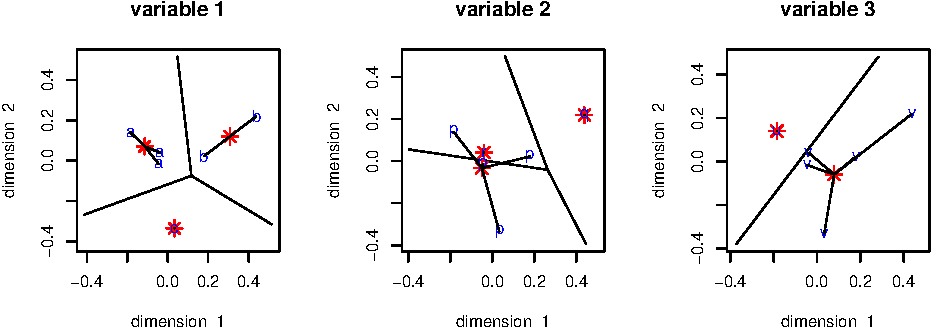
\includegraphics{smacofHO_files/figure-latex/smallhomals-1.pdf}

\begin{verbatim}
##       [,1] [,2] [,3]
##  [1,]    1    0    1
##  [2,]    1    1    1
##  [3,]    1    1    1
##  [4,]    1    0    1
##  [5,]    1    0    1
##  [6,]    1    1    1
##  [7,]    1    0    1
##  [8,]    1    1    1
##  [9,]    1    1    1
## [10,]    1    1    1
\end{verbatim}

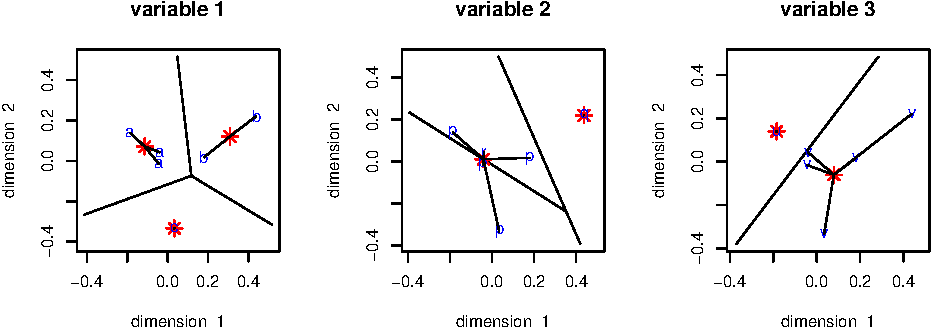
\includegraphics{smacofHO_files/figure-latex/small00-1.pdf}

\begin{verbatim}
##       [,1] [,2] [,3]
##  [1,]    1    0    1
##  [2,]    1    1    1
##  [3,]    1    1    1
##  [4,]    1    0    1
##  [5,]    1    0    1
##  [6,]    1    1    1
##  [7,]    1    0    1
##  [8,]    1    1    1
##  [9,]    1    1    1
## [10,]    1    1    1
\end{verbatim}

Stress is \ensuremath{1.1313536\times 10^{-9}} after 169 iterations.

\begin{center}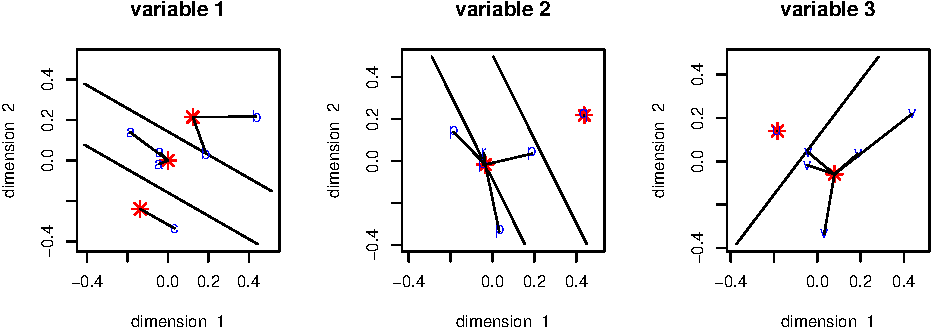
\includegraphics{smacofHO_files/figure-latex/small10-1} \end{center}

\begin{verbatim}
##       [,1] [,2] [,3]
##  [1,]    1    1    1
##  [2,]    1    1    1
##  [3,]    1    1    1
##  [4,]    1    1    1
##  [5,]    0    0    1
##  [6,]    1    1    1
##  [7,]    1    1    1
##  [8,]    1    1    1
##  [9,]    1    1    1
## [10,]    1    1    1
\end{verbatim}

Stress is \ensuremath{4.3071361\times 10^{-10}} after 73 iterations.

\subsection{Cetacea}\label{cetacea}

\subsection{Senate}\label{senate}

\subsection{GALO}\label{galo}

\section{Generalizations}\label{generalizations}

\begin{enumerate}
\def\labelenumi{\arabic{enumi}.}
\tightlist
\item
  Fuzzy Indicators
\item
  Voronoi with general sites
\end{enumerate}

\section*{References}\label{references}
\addcontentsline{toc}{section}{References}

\phantomsection\label{refs}
\begin{CSLReferences}{1}{0}
\bibitem[\citeproctext]{ref-deleeuw_C_23}
De Leeuw, J. 1923. {``Deconstructing Multiple Correspondence Analysis. Essays in Honour of Shizuhiko Nishisato.''} In \emph{Analysis of Categorical Data from Historical Perspectives}, edited by Eric J. Beh, Rosaria Lombardo, and Jose G. Clavel, 383--407. Springer.

\bibitem[\citeproctext]{ref-deleeuw_A_77}
---------. 1977. {``Correctness of Kruskal's Algorithms for Monotone Regression with Ties.''} \emph{Psychometrika} 42: 141--44.

\bibitem[\citeproctext]{ref-deleeuw_C_14}
---------. 2014. {``{History of Nonlinear Principal Component Analysis}.''} In \emph{{The Visualization and Verbalization of Data}}, edited by J. Blasius and M. Greenacre. Chapman; Hall.

\bibitem[\citeproctext]{ref-deleeuw_heiser_C_80}
De Leeuw, J., and W. J. Heiser. 1980. {``Multidimensional Scaling with Restrictions on the Configuration.''} In \emph{Multivariate Analysis, Volume {V}}, edited by P. R. Krishnaiah, 501--22. Amsterdam, The Netherlands: North Holland Publishing Company.

\bibitem[\citeproctext]{ref-deleeuw_mair_A_09a}
De Leeuw, J., and P. Mair. 2009. {``{Homogeneity Analysis in {R}: the Package homals}.''} \emph{Journal of Statistical Software} 31 (4): 1--21. \url{https://www.jstatsoft.org/v31/i04/}.

\bibitem[\citeproctext]{ref-gifi_B_80}
Gifi, A. 1980. \emph{Niet-Lineaire Multivariate Analyse {[}Nonlinear Multivariate Analysis{]}}. Leiden, The Netherlands: Department of Data Theory FSW/RUL.

\bibitem[\citeproctext]{ref-gifi_B_90}
---------. 1990. \emph{Nonlinear Multivariate Analysis}. New York, N.Y.: Wiley.

\bibitem[\citeproctext]{ref-heiser_deleeuw_A_79}
Heiser, W. J., and J. De Leeuw. 1979. {``Metric Multidimensional Unfolding.''} \emph{Methoden En Data Nieuwsbrief SWS/VVS} 4: 26--50.

\bibitem[\citeproctext]{ref-kruskal_64a}
Kruskal, J. B. 1964a. {``{Multidimensional Scaling by Optimizing Goodness of Fit to a Nonmetric Hypothesis}.''} \emph{Psychometrika} 29: 1--27.

\bibitem[\citeproctext]{ref-kruskal_64b}
---------. 1964b. {``{Nonmetric Multidimensional Scaling: a Numerical Method}.''} \emph{Psychometrika} 29: 115--29.

\bibitem[\citeproctext]{ref-michailidis_deleeuw_A_98}
Michailidis, G., and J. De Leeuw. 1998. {``The Gifi System for Descriptive Multivariate Analysis.''} \emph{Statistical Science} 13: 307--36.

\end{CSLReferences}

\end{document}
